% (1) Validation Engine
% - Join (Size of the dataset (#samples), Number of different nodes (#nodes), Number of Constraints (#constraints))
% - Reducing the SHACL Shape Schema to (#Constraints, #Constraints/Shape, #Targets of Target Shape (+ Reduced #Targets), #Reduced Number of Shapes needed to validate (shapes may be evaluate more the once))
%    - Shrink the number of Targets Validated (star-shape)
%    - Shrink the number of Shapes Validated over the Knowledge Graph
%    - Avoid Reevaluation of SHACL shapes used by multiple constraints (star-shape)

This section aims to experimentally evaluate the validation engine by using the synthetically generated benchmark setups in \textit{Synthetic Data A} and \textit{Synthetic Data B}. \textit{Synthetic Data A} provides knowledge graphs and different shape schemas, which will allow answering the research question \textbf{Q2}. \textit{Synthetic Data B} provides a dataset, the sample-to-node mapping as well as the entity validation function, which will be used to evaluate the join strategy (see section \ref{section_executing_the_join}). Both benchmarks will lead to an answer to the research question \textbf{Q1}.
Evaluating the validation engine in two parts by answering \textbf{Q1} and \textbf{Q2} is natural, as can be seen in algorithm \ref{algo:validation_engine}; the SHACL constraint validation is performed first (line \ref{algo:validation_engine:performShaclValidation}) and the constraint evaluation (line \ref{algo:validation_engine:call_evaluateConstraints}), which in case of data constraints reduces to the execution of the join, follows.

\subsection{SHACL Constraint Validation}
\label{section_evaluation_validation_engine_shacl}
An ablation study based on nine different test beds of \textit{Synthetic Data A} is performed to show the effects of the heuristics proposed in section \ref{section_shaclapi}. Therefore, the execution time of the SHACL constraint validation (e.g., applying the heuristics, running the SHACL engine, collecting the SHACL validation results) and the number of SHACL validation results generated in the process are measured.

The study is split into two parts: In the first part, only a single constraint of each test bed is evaluated over the dataset extracted from the knowledge graph. In the second part, all constraints as shown in Figure \ref{fig:class_venn_diagram_eval} are evaluated. Figure \ref{fig:metrics_ablation_single} presents the results of the first part of the ablation study (with none as the baseline). The results of the second part of the ablation study are shown in Figure \ref{fig:metrics_ablation} with the baseline separately shown in table \ref{fig:baseline_multiple_constraints}. Based on the results, the impact of the heuristics is discussed.

\begin{figure}
        \centering
        \begin{subfigure}{\linewidth}
            \centering
            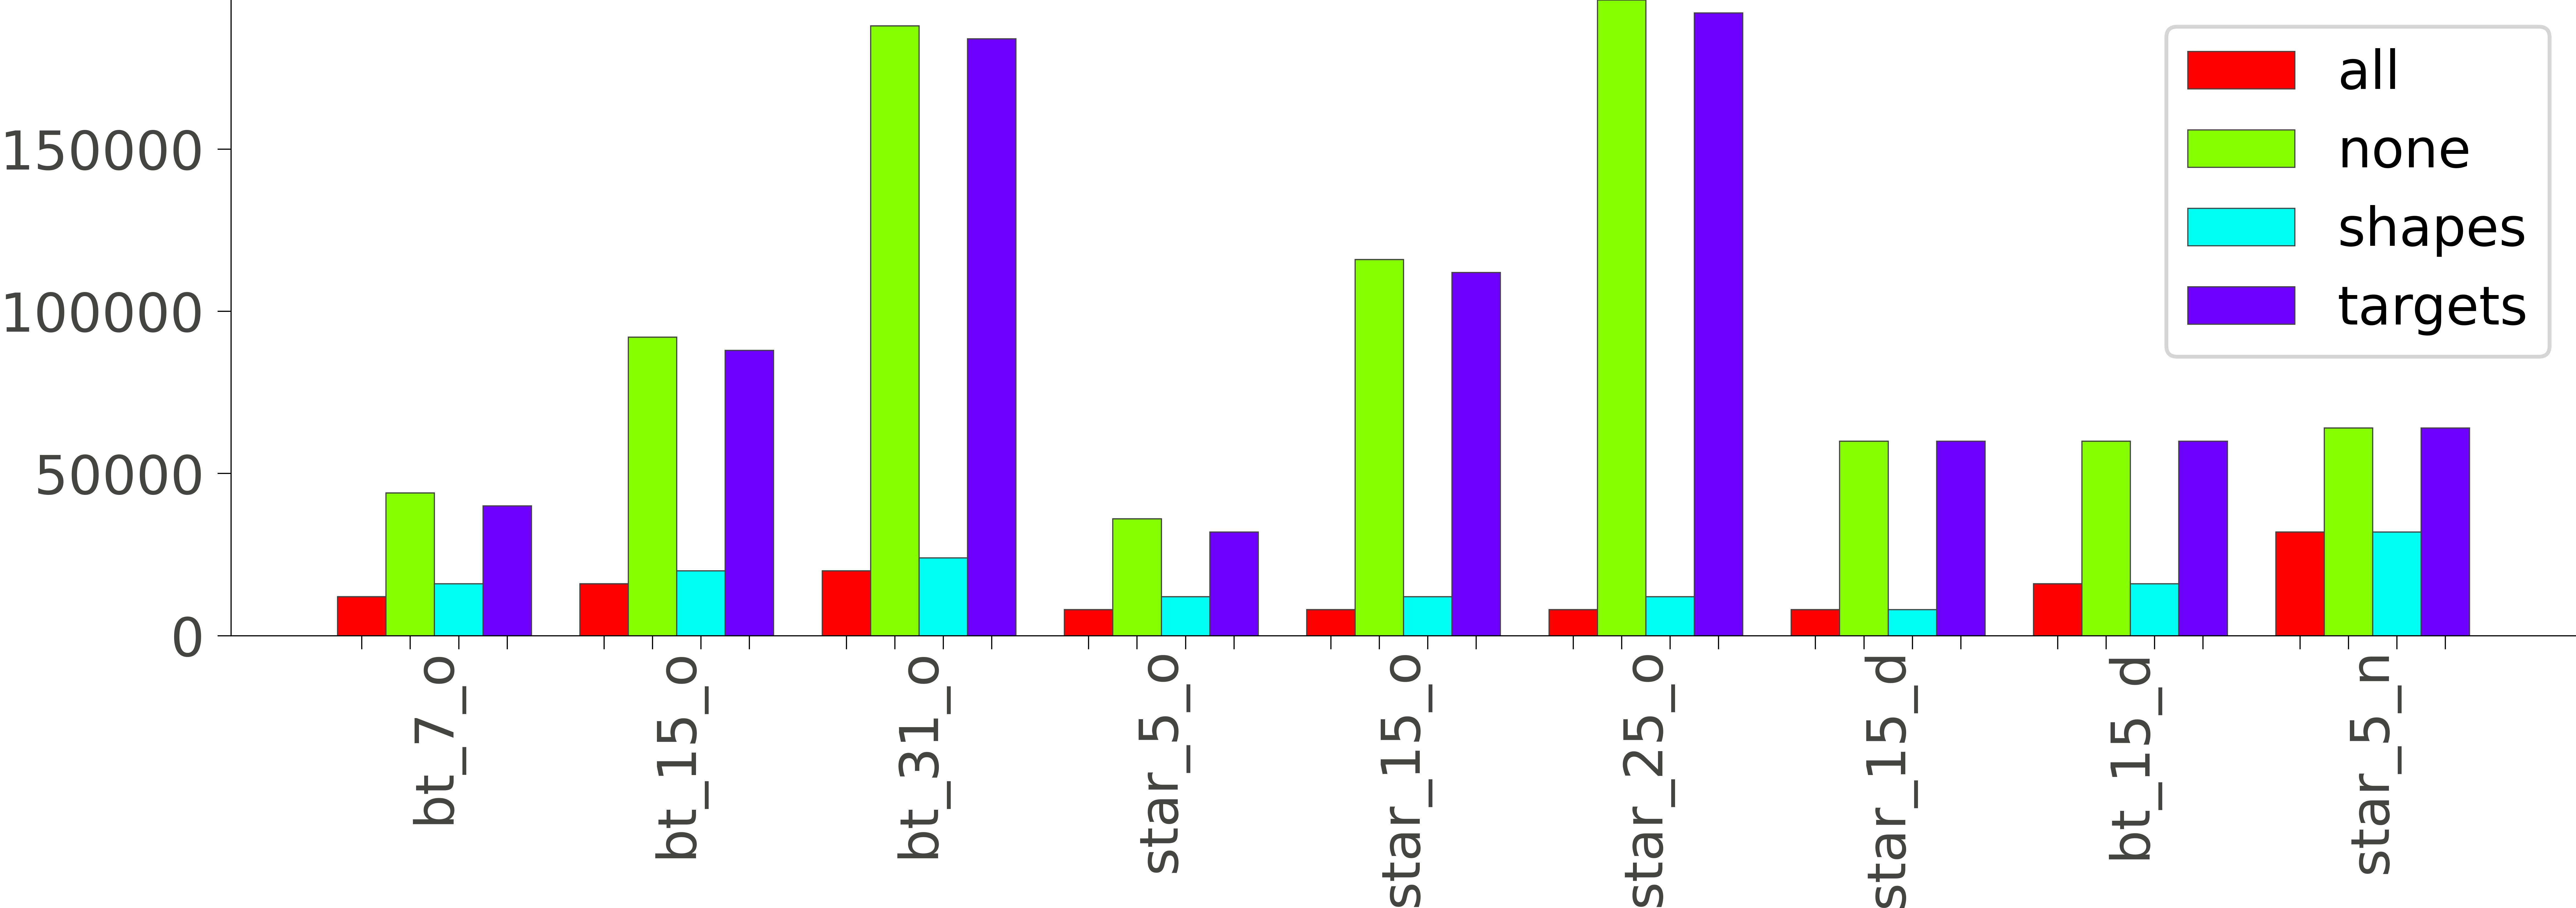
\includegraphics[width=\textwidth]{images/evaluation/ablation_study_targets_single.png}
            \caption{Number of SHACL validation results}
            \label{fig:number_of_shacl_validation_results_single}
        \end{subfigure}
        \vspace{0.3cm}
        \begin{subfigure}{\linewidth}
            \centering
             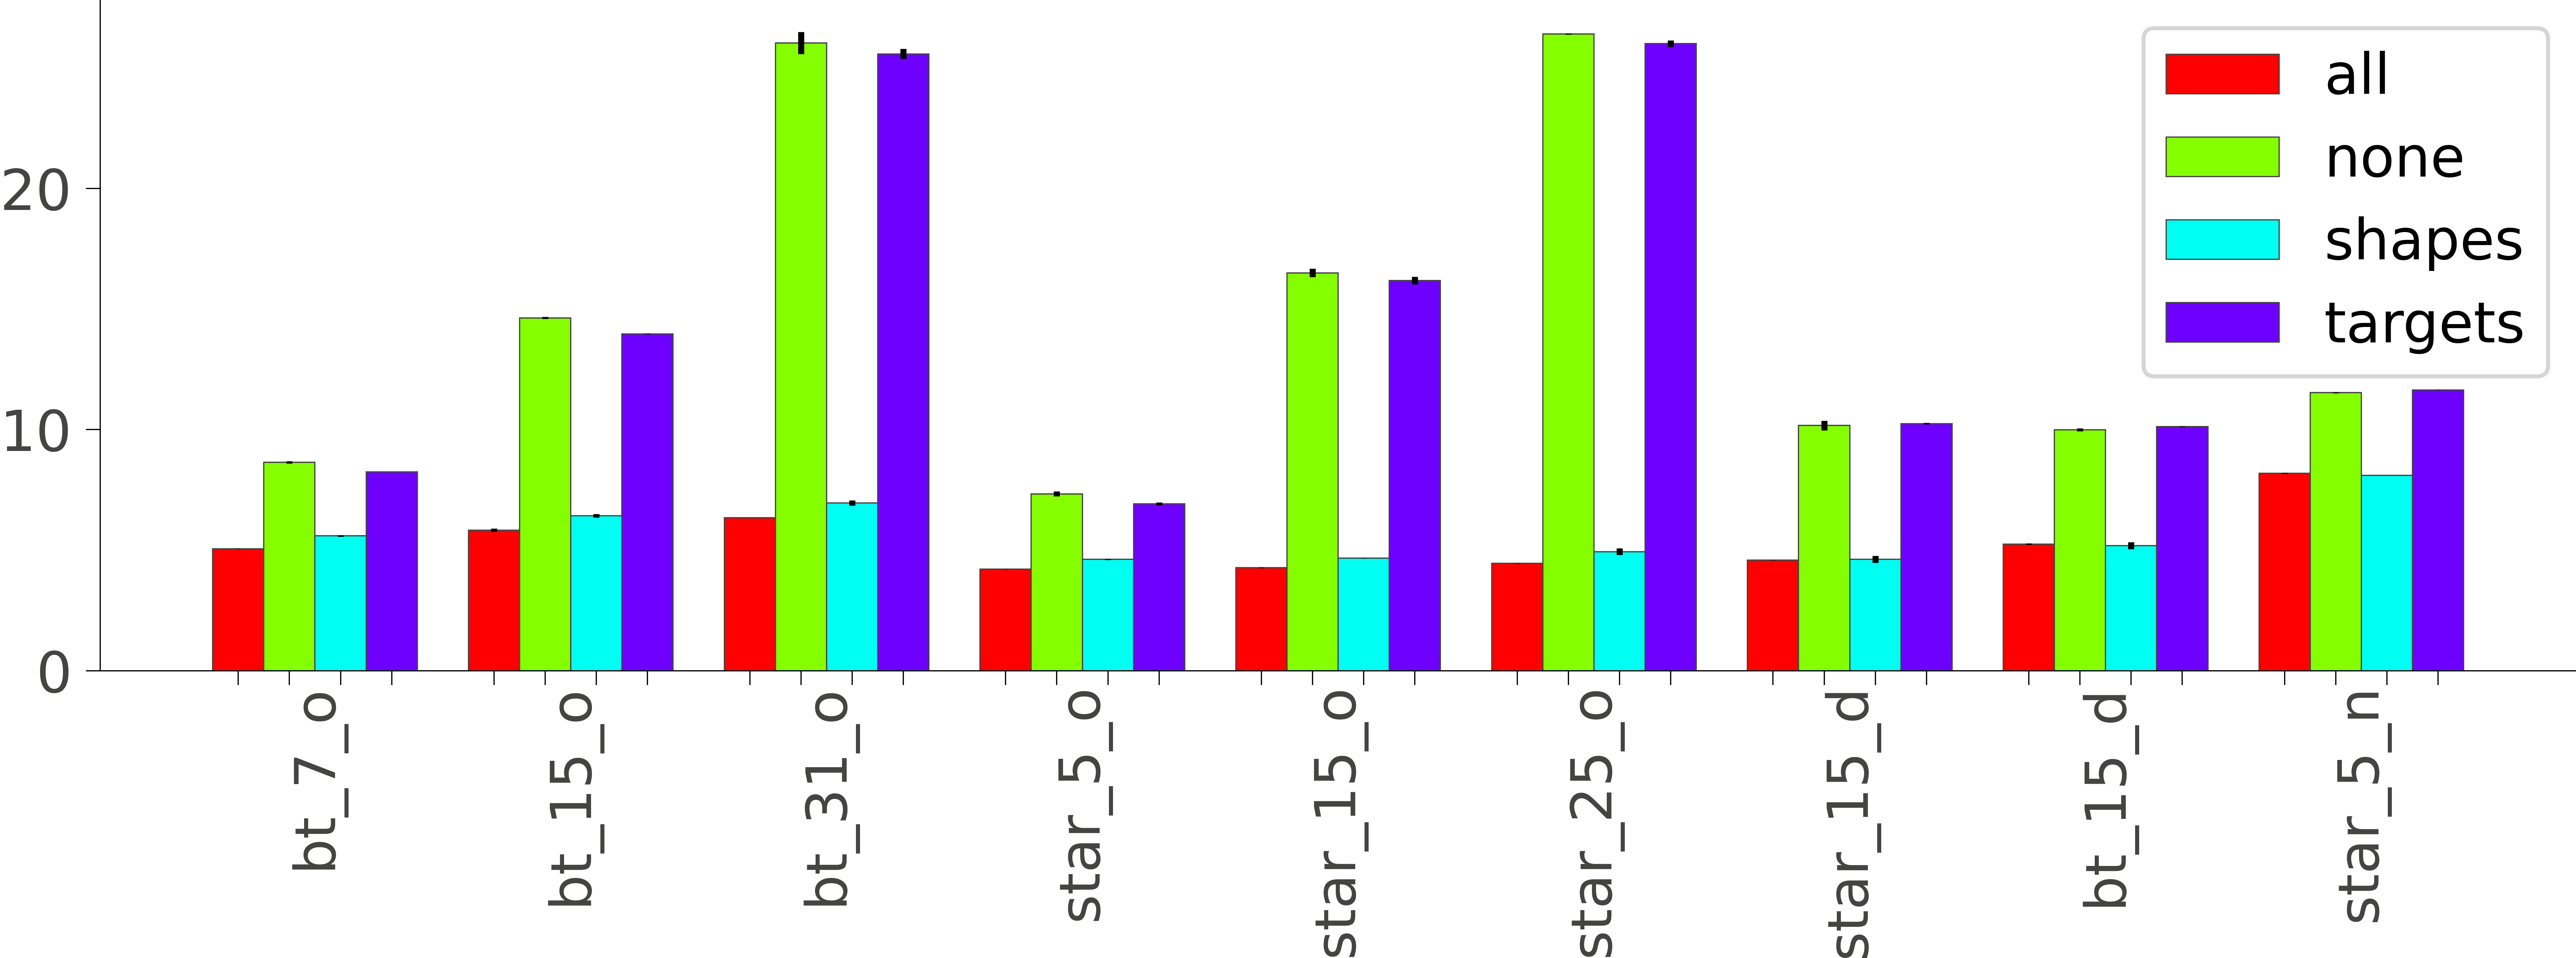
\includegraphics[width=\textwidth]{images/evaluation/ablation_study_shacl_time_single.png}
            \caption{Execution time [s]}
            \label{fig:average_execution_time_shacl_single}
        \end{subfigure} 
        \caption{Metrics observed during the execution of the validation engine on performing the SHACL validation of a single constraint in nine test beds of \textit{Synthetic Data A}. none - the baseline does not make use of any heuristics, shapes - the shape network is pruned, targets - the target reduction is applied, all - combination of shapes and targets}
        \label{fig:metrics_ablation_single}
\end{figure}

\begin{figure}
        \centering
        \begin{subfigure}{\linewidth}
            \centering
            
\includegraphics[width=\textwidth]{images/evaluation/ablation_study_targets.png}
            \caption{Number of SHACL validation results}
            \label{fig:number_of_shacl_validation_results}
        \end{subfigure}
        \vspace{0.3cm}
        \begin{subfigure}{\linewidth}
            \centering
    
\includegraphics[width=\textwidth]{images/evaluation/ablation_study_shacl_time.png}
            \caption{Execution time [s]}
            \label{fig:average_execution_time_shacl}
        \end{subfigure} 
        \caption{Metrics observed during the execution of the validation engine on performing the SHACL validation of all constraints in nine test beds of \textit{Synthetic Data A}. simult. - constraints are validated simultaneously, shapes - the shape network is pruned, targets - the target reduction is applied, all - combination of simult., shapes and targets}
        \label{fig:metrics_ablation}
\end{figure}

\begin{table}
    \centering
    \begin{tabular}{llll|lllll}
        \toprule
        \multicolumn{4}{c|}{bt} & \multicolumn{5}{c}{star}\\
        7\_o & 15\_o & 31\_o & 15\_d & 5\_o & 15\_o & 25\_o & 15\_d & 5\_n\\
        \midrule
        \midrule
         34.6 & 117.0 & 416.5 & 79.9 & 29.3 & 231.0 & 633.6 & 142.4 & 46.1\\
        \bottomrule
    \end{tabular}
    \caption{Execution time [s] observed during the execution of the validation engine on performing the SHACL validation of all constraints in 9 test beds of \textit{Synthetic Data A} without using any heuristic.}
    \label{fig:baseline_multiple_constraints}
\end{table}


\paragraph{Prune Shape Network} refers to the heuristic proposed in lemma \ref{S:removeShapes} and excels in reducing the number of SHACL validation results needed to be generated in the first part of the ablation study. That is because in both shape schema topologies used, the number of shapes can be reduced, when only validating a single constraint. In the star-shaped case, the reduction is theoretically able to remove $(K - 1)$ shapes leaving $2$ shapes in the network, and in the binary-tree-shaped case even $2 * (K - 1) - \log_2(K)$ shapes leaving $\log_2(K) + 1$ shapes in the network. In the \glqq overlap\grqq{}-case, the number of SHACL validation results can be estimated to be $(\text{\#shapes} * 4,000 + K * 4,000)$. Therefore, the total number of SHACL validation results in the \glqq overlap\grqq{} case is reduced from $(K + 1) * 4,000 + K * 4,000$ resp. $(2*K - 1) * 4,000 + K * 4,000$ in the baseline case (e.g., not using any heuristic) to $2 * 4,000 + 4,000$ resp. $(\log_2(K) + 1) * 4,000 + K * 4,000$ when only pruning the shape network. The proactive reader might calculate the theoretical reduction of the number of SHACL validation results with the formula for the \glqq distinct\grqq{}-case $\text{\#shapes} * 4,000$ and the \glqq nested\grqq{}-case $(\text{\#shapes} - K) * 4,000 + \sum_i^K (4,000 + (i - 1) * 2,000)$. 
As it turns out, the theoretical numbers exactly match the estimated numbers in Figure \ref{fig:number_of_shacl_validation_results_single}, which proves the functionality of the heuristic for the given test beds. Comparing the results in figures \ref{fig:metrics_ablation} and \ref{fig:metrics_ablation_single} shows a strong correlation between the number of SHACL validation results and the execution time; emphasizing the importance of the shape network pruning when possible. In the second part of the ablation study, the shape network pruning does not impact as none of the shape schemas can be reduced. 

\paragraph{Target Reduction} refers to the heuristic proposed in lemma \ref{S:removeTargets}. Both, in the first part and in the second part of the ablation study, the target reduction impacts and reduces the number of targets of the target shapes given by the constraints. Precisely, in the first part of the ablation study, in the \glqq overlap\grqq{}-case, the target reduction exactly removes the $4,000$ additional entities included in the target definition of the shape but not included in $Qs$. This scales in the second part of the ablation study to $K * 4,000$ as for each constraint $4,000$ entities were validated without being included in the seed nodes. In the \glqq distinct\grqq{}- and \glqq nested\grqq{}-case, the set of entities $Qs$ includes all the entities in the target definitions of the shapes, which is why the target reduction does not have a further impact and the number SHACL validation results stay the same in all cases. Even though the target reduction was not able to reduce the number of SHACL validation results as much as the shape network pruning, it still impacts the average execution time as can be seen in figures \ref{fig:average_execution_time_shacl_single} and \ref{fig:average_execution_time_shacl}.

\paragraph{Simultaneous Constraint Validation} refers to the heuristic proposed in lemma \ref{S:simulataneous_constraint_validation} and, therefore, only applies to cases in which multiple constraints are given, which is not the case in the first part of the ablation study. However, it excels in the second part by preventing the SHACL engine to produce redundant validation results. Even if the heuristics above are able to reduce the number of SHACL validation results needed, still shapes are processed multiple times when validating each constraint on its own. All setups in Figure \ref{fig:metrics_ablation} make use of the heuristics except for the \glqq shapes + targets\grqq{}-configuration. Therefore, Figure \ref{fig:number_of_shacl_validation_results} shows the impact of the simultaneous constraint validation on the number of SHACL validation results. In theory, the impact can be calculated as follows: In the case of the star-shaped shape schemas, shape $0$ is validated $K$ times over the knowledge graph, and in the case of the binary tree, a shape at depth $i$ is validated $2^{(h-i)}$ times. This is the reason for the additional SHACL validation results, which the \glqq shapes + targets\grqq{}-configuration generates in comparison to the \glqq all\grqq{}-configuration.
Although the two heuristics perform well compared to the baseline, still the shaclAPI needs to apply the heuristics above unnecessarily often, the SHACL validation is performed with smaller and more queries and the validation engine needs to manage unnecessary validation results. All these components contribute to a comparatively high execution time of the \glqq shapes + targets\grqq{}-configuration in Figure \ref{fig:average_execution_time_shacl}.


\paragraph{Conclusion} The preceding discussion leads to an answer to the research question \textbf{Q2}. Given the nine test beds, pruning the shape network alone reduced the execution time by 65\% on average, while reducing the target definition of the target shapes only reduced the execution time by 3\% on average. The simultaneous constraint validation was able to improve the average execution time by 90\%. Applying all heuristics reduced the execution time by 94\% on average. Further, the number of SHACL validation results strongly correlates with the execution time and whether the heuristic was able to reduce the number of actions (e.g., queries to the endpoint) of the SHACL engine. All heuristics proposed in section \ref{section_shaclapi} at least impact on the execution time of the SHACL validation in the same order of magnitude they were able to shrink the number of SHACL validation results. However, this depends on the knowledge graph and the SHACL shape schema. Additionally, figures \ref{fig:metrics_ablation} and \ref{fig:metrics_ablation_single} show that in cases the heuristics do not apply, it also does not impact negatively in the given test beds.

\subsection{The Join Strategy}
\label{section_evaluation_validation_engine_join}

In section \ref{section_executing_the_join} two different join strategies were presented: 

\begin{description}
\item[\textbf{A)} Join T at the end.] The SHACL validation results are first joined together before being linked to the dataset via the sample-to-node mapping. The two join heuristics (see lemma \ref{S:join_heuristic1} and \ref{S:join_heuristic2}) propose to use this approach to keep intermediate results as small as possible and, in turn, minimize the execution time of the join operations in Figure \ref{fig:join_strategies_left_deep1}. However, full-outer-joins are required to keep all SHACL validation results. The implementation of lemma \ref{S:join_heuristic1} was described in section \ref{section_performance_efficiency}.  
\item[\textbf{B)} Join T at the beginning.] The SHACL validation results are directly joined with the dataset via the sample-to-node mapping. The intermediate results are always as large as possible, but only left-outer joins are required to keep all samples in the dataset. Furthermore, this strategy can be used when joined SHACL results are needed early.
\end{description}

In the first step, the \textit{Synthetic Data B} benchmark is used for a load test of the implementation. Therefore, the number of samples, nodes, or constraints are varied, to see the effect of each of the parameters of the test bed on the execution time of the join strategy. Figure \ref{fig:load_test_join} presents the results in terms of execution time. 

\begin{figure}
    \centering
    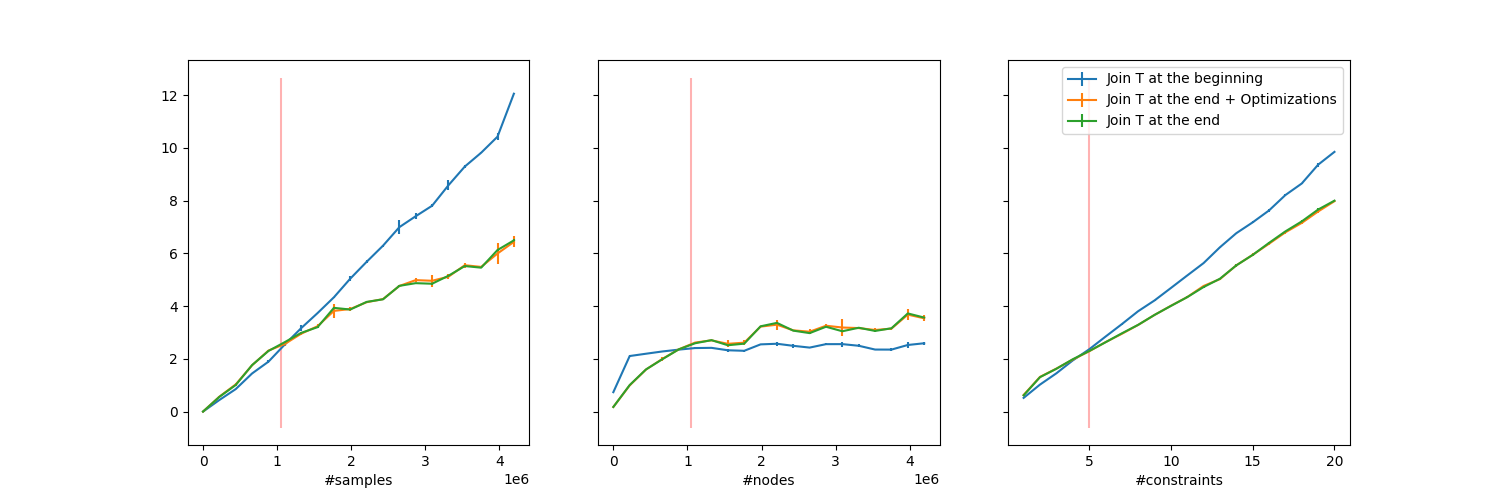
\includegraphics[trim=70 10 70 20,clip, width=\textwidth]{images/evaluation/join_exp.png}
    \caption{Execution time [s] of the different join strategies observed during the execution of the validation engine on performing different join strategies for test beds of \textit{Synthetic Data B} with a varied number of samples (\#samples), number of seed nodes (\#nodes) or number of constraints (\#constraints). The vertical red line marks the default value of the varied parameter as shown in table \ref{fig:parameters_used_to_generate_the_custom_dataset}}
    \label{fig:load_test_join}
\end{figure}

Varying the number of samples increases the time spent on joining with strategy \textbf{A} and \textbf{B} in a roughly linear fashion. In the case of strategy \textbf{A} resp. \textbf{B} the execution time raises approximately by $1.38$ resp. $2.75$ seconds per million samples. However, a small number of samples results in a larger portion of unique nodes in the sample-to-node mapping in relation to the number of samples, and strategy \textbf{B} turns out to be faster. Similar behavior can be seen when varying the number of seed nodes: Raising the number of seed nodes and, therefore, increasing the portion of unique nodes in the sample-to-node mapping in relation to the number of samples, strategy \textbf{B} is faster. In the opposite case, strategy \textbf{A} is faster. Varying the number of constraints scales the execution time in a linear fashion. %, which is logical as effectively the number of operations in the execution tree of the join operation is varied. 
Finally, one can observe that the further optimizations to decrease the cardinality of the intermediate results do not impact in case of the given benchmark. 

Both observations may be due to the random nature of \textit{Synthetic Data B}: A large portion of unique nodes makes overlapping of entities of the SHACL validation results unlikely. On the other hand, a small to moderate portion of unique nodes makes overlapping more probable. However, the random nature of the experiment is not natural. In the real world, the entities often match or overlap (e.g., multiple constraints about different person types) or are nested into each other (e.g., constraints becoming more specific about a protocol).

This motivates the \textit{Synthetic Data A} benchmark, in which entities are distributed to classes and the SHACL validation results are not generated by a random process and assigned to a random subset of the seed nodes. This is the second step of the evaluation of the join strategy to validate the behavior observed in the preceding benchmark. The results are depicted in Figure \ref{fig:scenario_test_join}.

\begin{figure}
        \centering
        \begin{subfigure}{\linewidth}
            \centering
            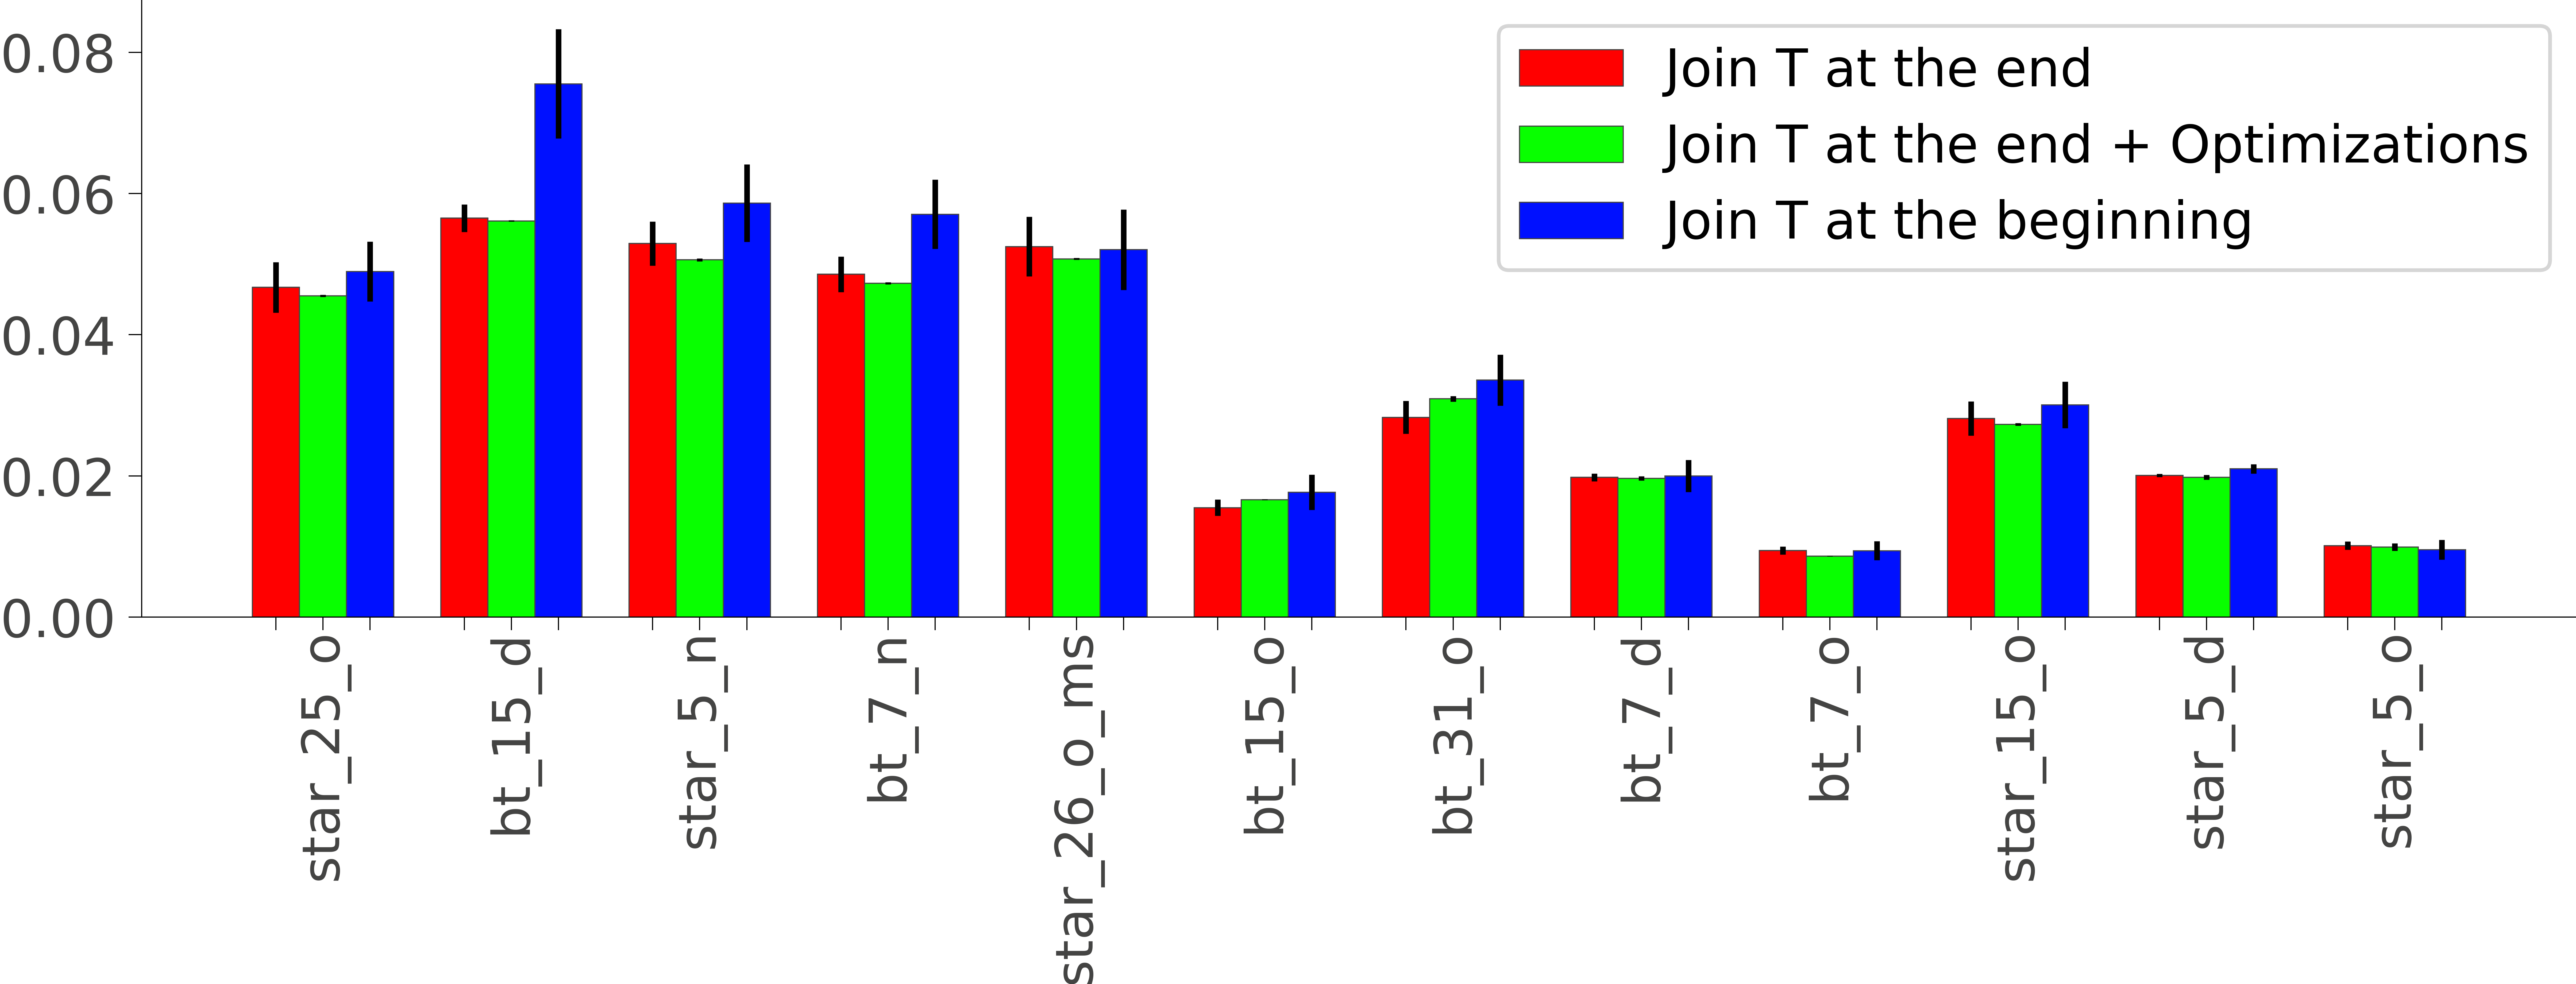
\includegraphics[width=\textwidth]{images/evaluation/validation_engine_join_small.png}
            \caption{Cheap Joins}
            \label{fig:scenario_test_join_small}
        \end{subfigure}
        \vspace{0.3cm}
        \begin{subfigure}{\linewidth}
            \centering
    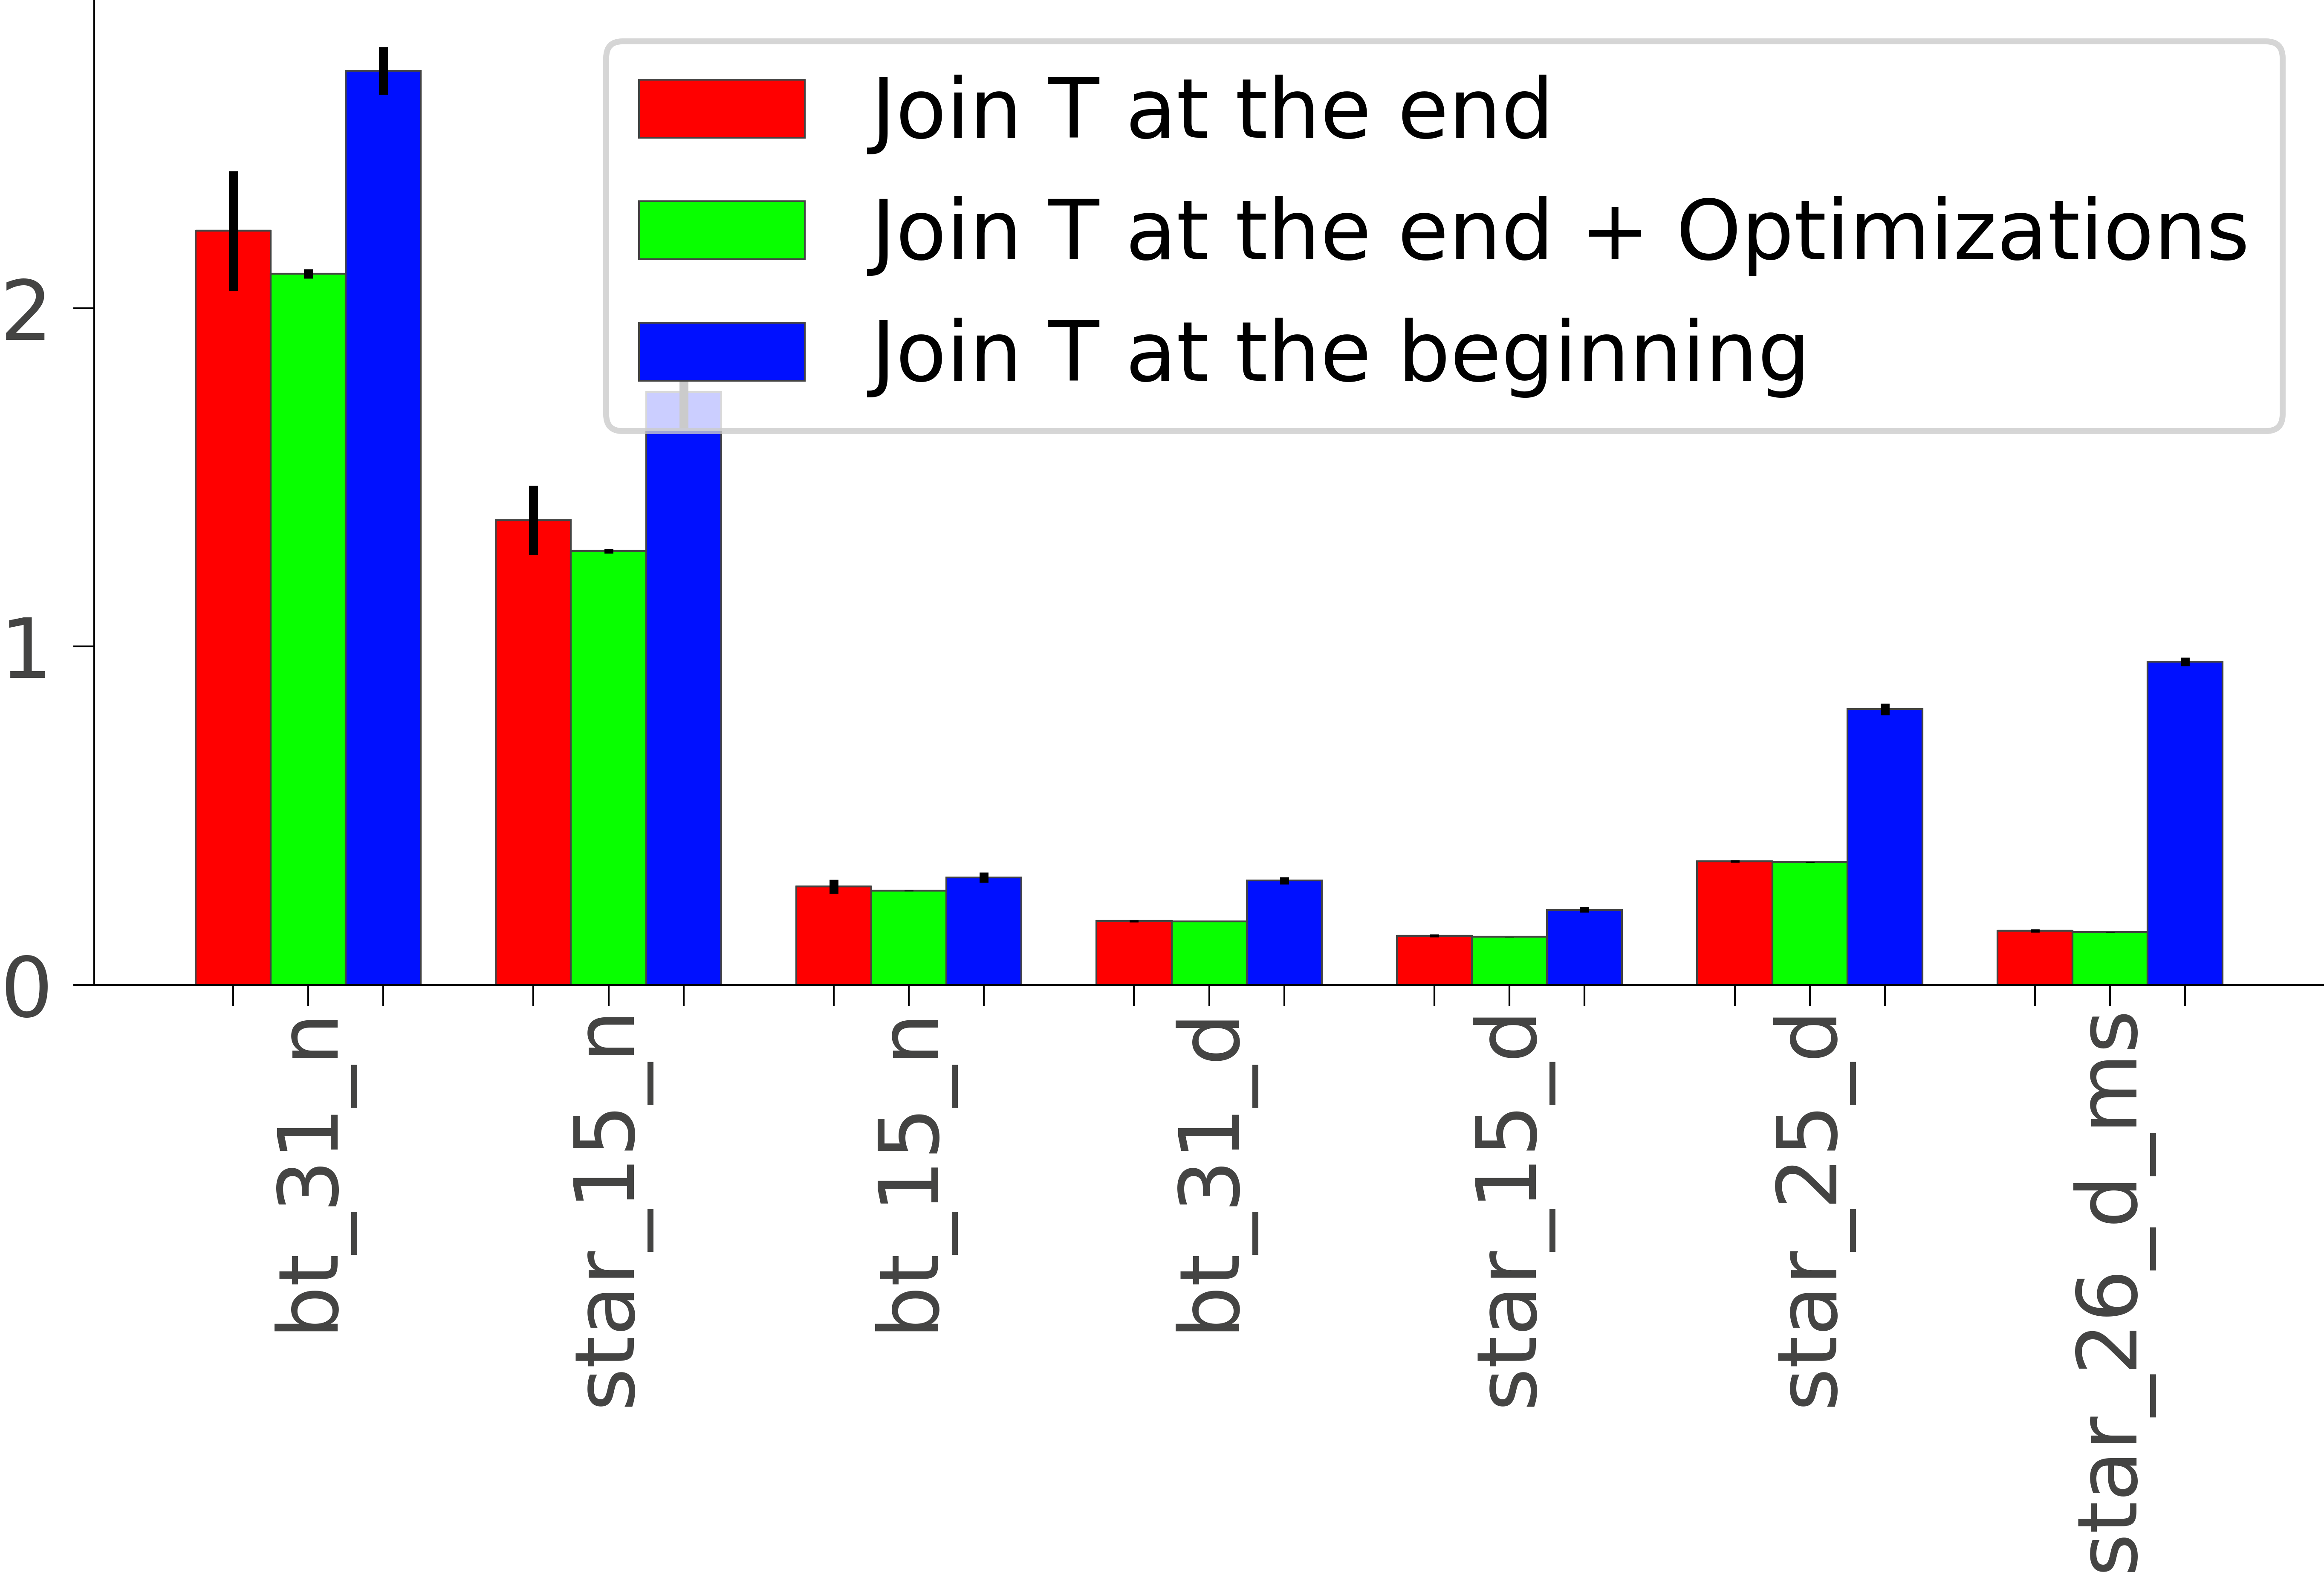
\includegraphics[width=0.5\textwidth]{images/evaluation/validation_engine_join_large.png}
        \caption{Expensive Joins}            \label{fig:scenario_test_join_large}
        \end{subfigure} 
    \caption{Execution time [s] observed during the execution of the validation engine on performing different join strategies for 19 different test beds of \textit{Synthetic Data A}. ms - marks a variation of the test bed, in which the target definition of five shapes each refer to the same class, Optimizations - The optimizations to reduce the number of intermediate results (see section \ref{section_performance_efficiency})}
    \label{fig:scenario_test_join}
\end{figure}


First of all, one can observe that strategy \textbf{B} performs worse or as good as strategy \textbf{A} without optimizations. A reason for that might be the nested or distinct class distributions of the entities to classes, which encourage constantly growing intermediate results. However, that is even true for the \glqq overlap\grqq{}-case in which the number of SHACL validation results is equal for all constraints. The latter can be due to the implementation of strategy \textbf{B} having a larger overhead in comparison to strategy \textbf{A}. That is because \textbf{B} has to use multiple pandas join calls where, on the other hand, \textbf{A} only requires a maximum of two calls. 

Next, one can observe that the optimizations impact differently depending on the distribution of entities to classes. However, the execution times generally seem to vary less in the optimized case. 


In the \glqq nested\grqq{}-case, it is necessary to order the SHACL validation results of the different target shapes according to their size to get constantly growing intermediate results during the execution of the join strategy. Therefore, the optimizations impact and the average execution time decreases by approximately $6\%$.

The test beds ending with ``\_ms'' are specially designed only to produce constantly growing intermediate results during the join when the SHACL validation results of the constraints with a target shape having the same class in their target definition are joined next to each other. However, the experiments do not show a difference in the execution time of strategy \textbf{A} when using the optimizations or not.

In the case of a distinct distribution, the intermediate results will constantly grow independent of the order in which the SHACL validation results are joined. Therefore, it is logical that the optimizations do not impact, and the average execution time of the join strategy is approximately the same in all of these test beds.

In the \glqq overlap\grqq{}-case, the order does not matter at all, and, as already noted, the intermediate results are of constant size independent of the join order. In this case, the optimization adds an unnecessary overhead (e.g., sorting by the number of SHACL validation results and grouping per target definition). Therefore, it can even lead to worse execution times, as observed in some cases. 

In summary, research question \textbf{Q1} can be answered: Join strategy \textbf{A} is indeed faster in cases where the distribution of entities to classes is chosen in a way that encourages the production of constantly growing intermediate results. The second part of the experiments even shows that in the case of a relatively small number of seed nodes, strategy \textbf{B} is slower in general. Further, optimizing the order of the join operations in an approach to keep the intermediate results small stabilizes the execution time of the join strategy. 